\chapter{Solución propuesta}
\label{ch:solucion}

La estimación de consumo energético asociada a firmware bare-metal requiere
combinar tres componentes que operan de forma coordinada sobre el CV32E40P:
un circuito de medición eléctrica que adquiere la potencia real consumida por la plataforma,
un módulo hardware integrado en el procesador que clasifica las instrucciones
ejecutadas y las acumula en contadores accesibles por CSR, y una etapa de
análisis de datos que relaciona ambas fuentes para obtener los coeficientes del
modelo energético. La Figura~\ref{fig:arquitectura_general} ilustra la
interacción entre los tres componentes.

\begin{figure}[H]
    \centering
    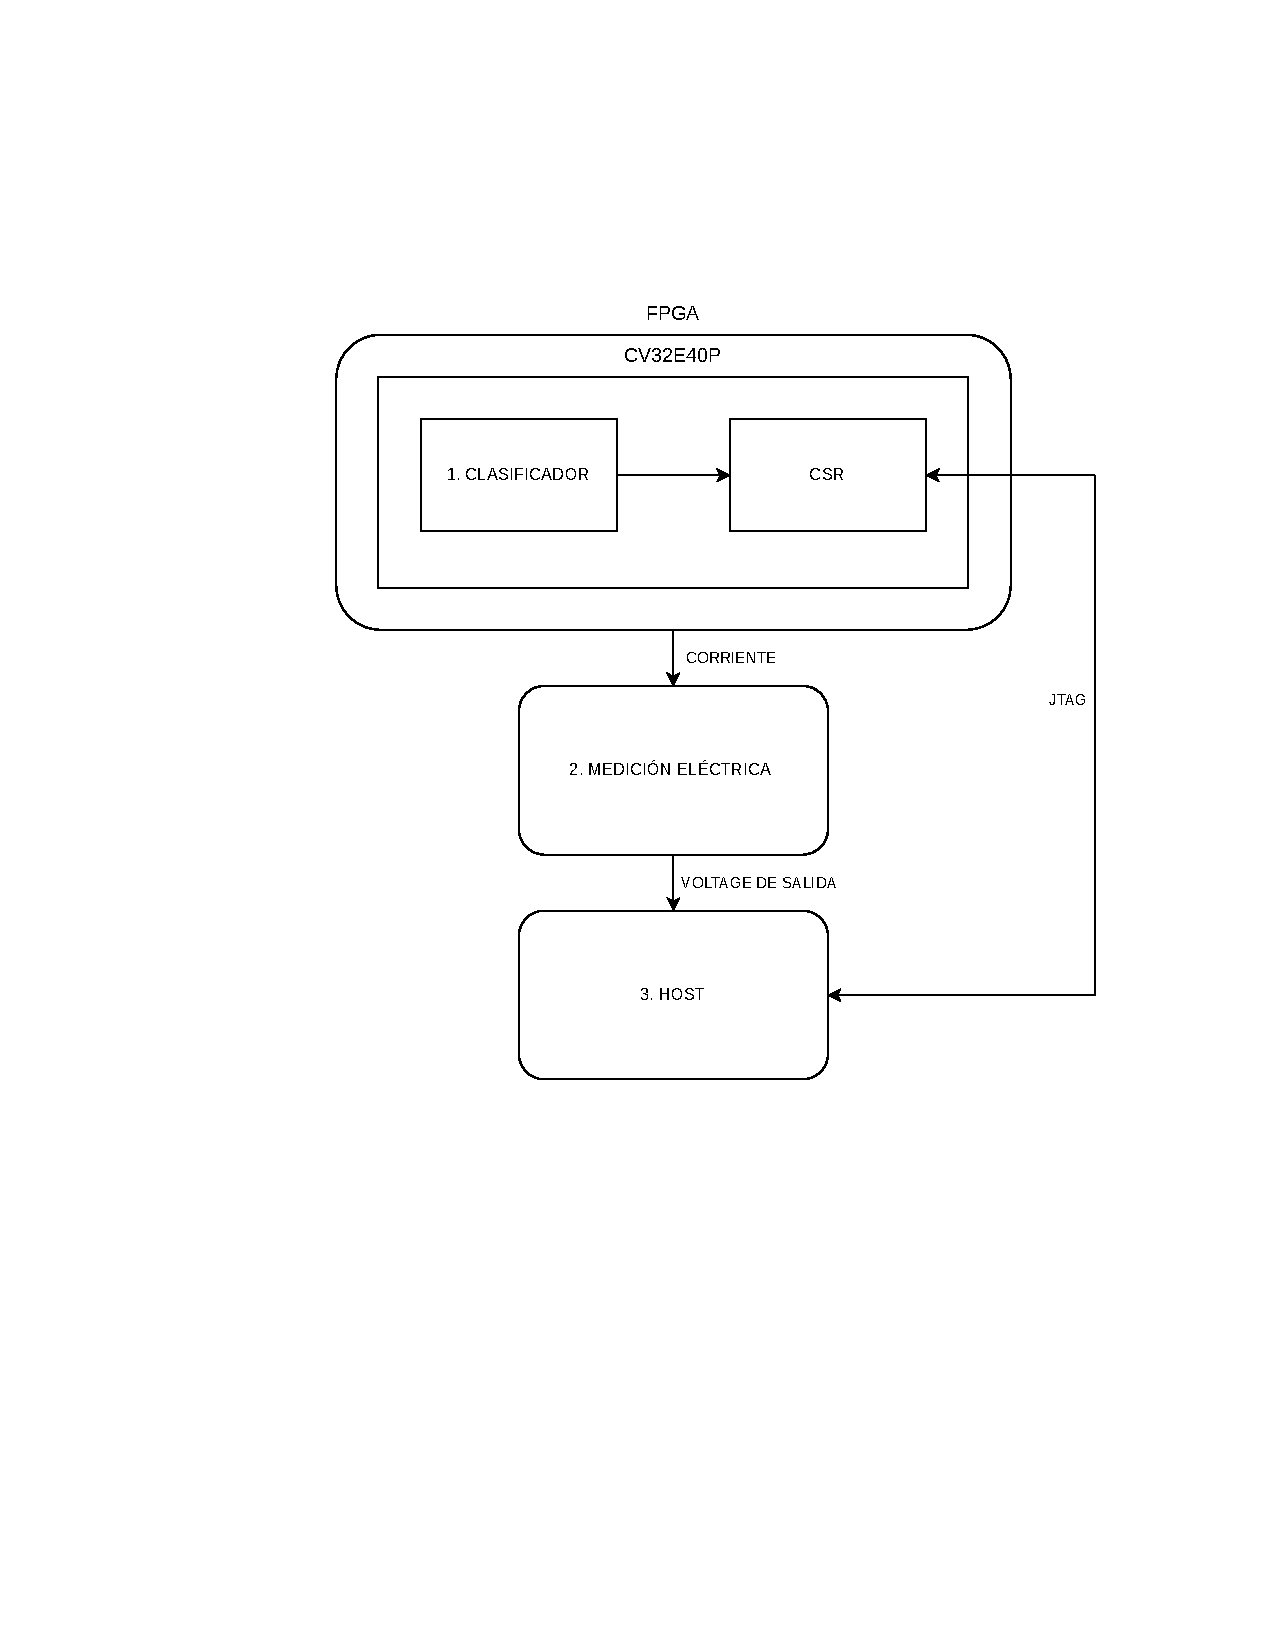
\includegraphics[width=0.70\textwidth, height=0.40\textheight, keepaspectratio,
        trim=135pt 245pt 55pt 125pt, clip]{fig/diagrama_3_1_arquitectura_general.pdf}
    \caption{Arquitectura general del sistema propuesto.}
    \label{fig:arquitectura_general}
\end{figure}

% -----------------------------------------------------------------------
\section{Medición de potencia}
\label{sec:medicion_potencia}

La potencia de referencia se obtiene midiendo la corriente en la línea de
alimentación de la Nexys~A7-100T durante la ejecución del SoC PULPissimo. Esta
medición corresponde al consumo observado en la plataforma FPGA completa bajo la
configuración experimental, no al consumo aislado del núcleo como circuito
independiente. La cadena de medición consta de un módulo de sensado basado en
INA240A1 con resistor de shunt integrado, un convertidor analógico-digital
ADS1115 y un sistema de adquisición autónomo que registra la tensión de salida
para su procesamiento posterior.

\subsection{Módulo de sensado de corriente}
\label{sec:modulo_sensado}

La medición de corriente se realiza con un módulo conectado en serie con la
línea de 5\,V del jack de alimentación de la placa. Este módulo integra el
amplificador INA240A1 y un resistor de shunt marcado como R100, equivalente a
$R_\text{shunt} = 100\,\text{m}\Omega$. La corriente demandada por la carga
genera sobre este resistor una caída de tensión proporcional~\cite{ti_current_sensing}:

\begin{figure}[H]
    \centering
    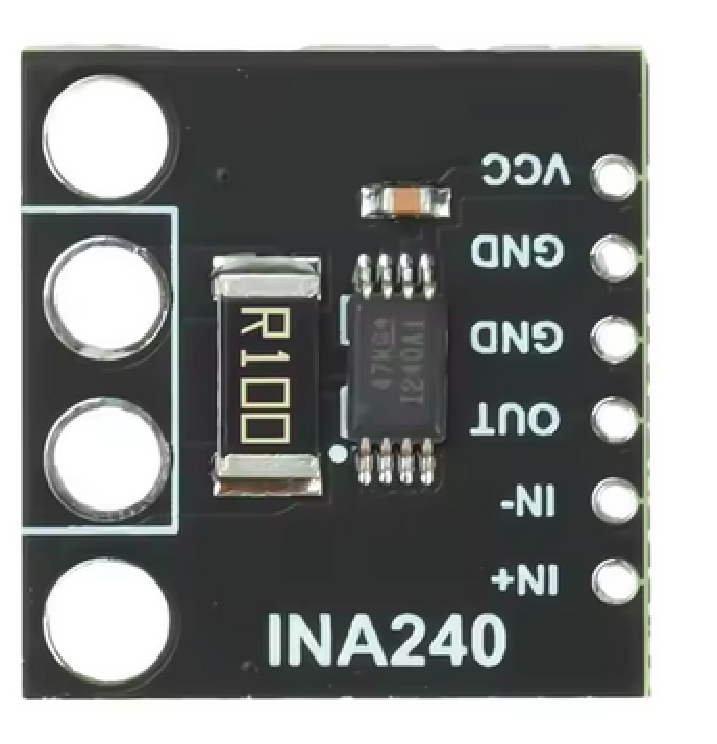
\includegraphics[width=0.35\textwidth]{fig/ina240_module.pdf}
    \caption{Módulo de sensado basado en INA240 con resistor de shunt integrado.}
    \label{fig:ina240_modulo}
\end{figure}

\begin{equation}
    V_{R_\text{shunt}} = I \cdot R_\text{shunt}
    \label{eq:vshunt}
\end{equation}

El valor de $R_\text{shunt}$ se eligió como compromiso entre perturbación de la
alimentación y resolución de medición. Para el consumo máximo de placa reportado
por la Nexys~A7-100T, 5\,W desde una fuente de 5\,V~\cite{nexysA7rm}, la
corriente es de 1\,A y la caída sobre el shunt es de 100\,mV, equivalente al
2\,\% de $V_{DD}$.

La potencia instantánea se obtiene como:

\begin{equation}
    P = V_{DD} \cdot \frac{V_{R_\text{shunt}}}{R_\text{shunt}}
    \label{eq:potencia_medida}
\end{equation}

El resistor se coloca en configuración \emph{high-side}, en serie entre la
fuente de alimentación y la carga, para medir directamente la corriente
entregada por la fuente a la Nexys~A7-100T~\cite{ti_current_sensing}. En esta
posición, la señal diferencial sobre el shunt queda superpuesta a la línea de
5\,V, por lo que el amplificador debe medir caídas pequeñas en presencia de un
voltaje de modo común cercano a la tensión de alimentación.


\begin{figure}[H]
    \centering
    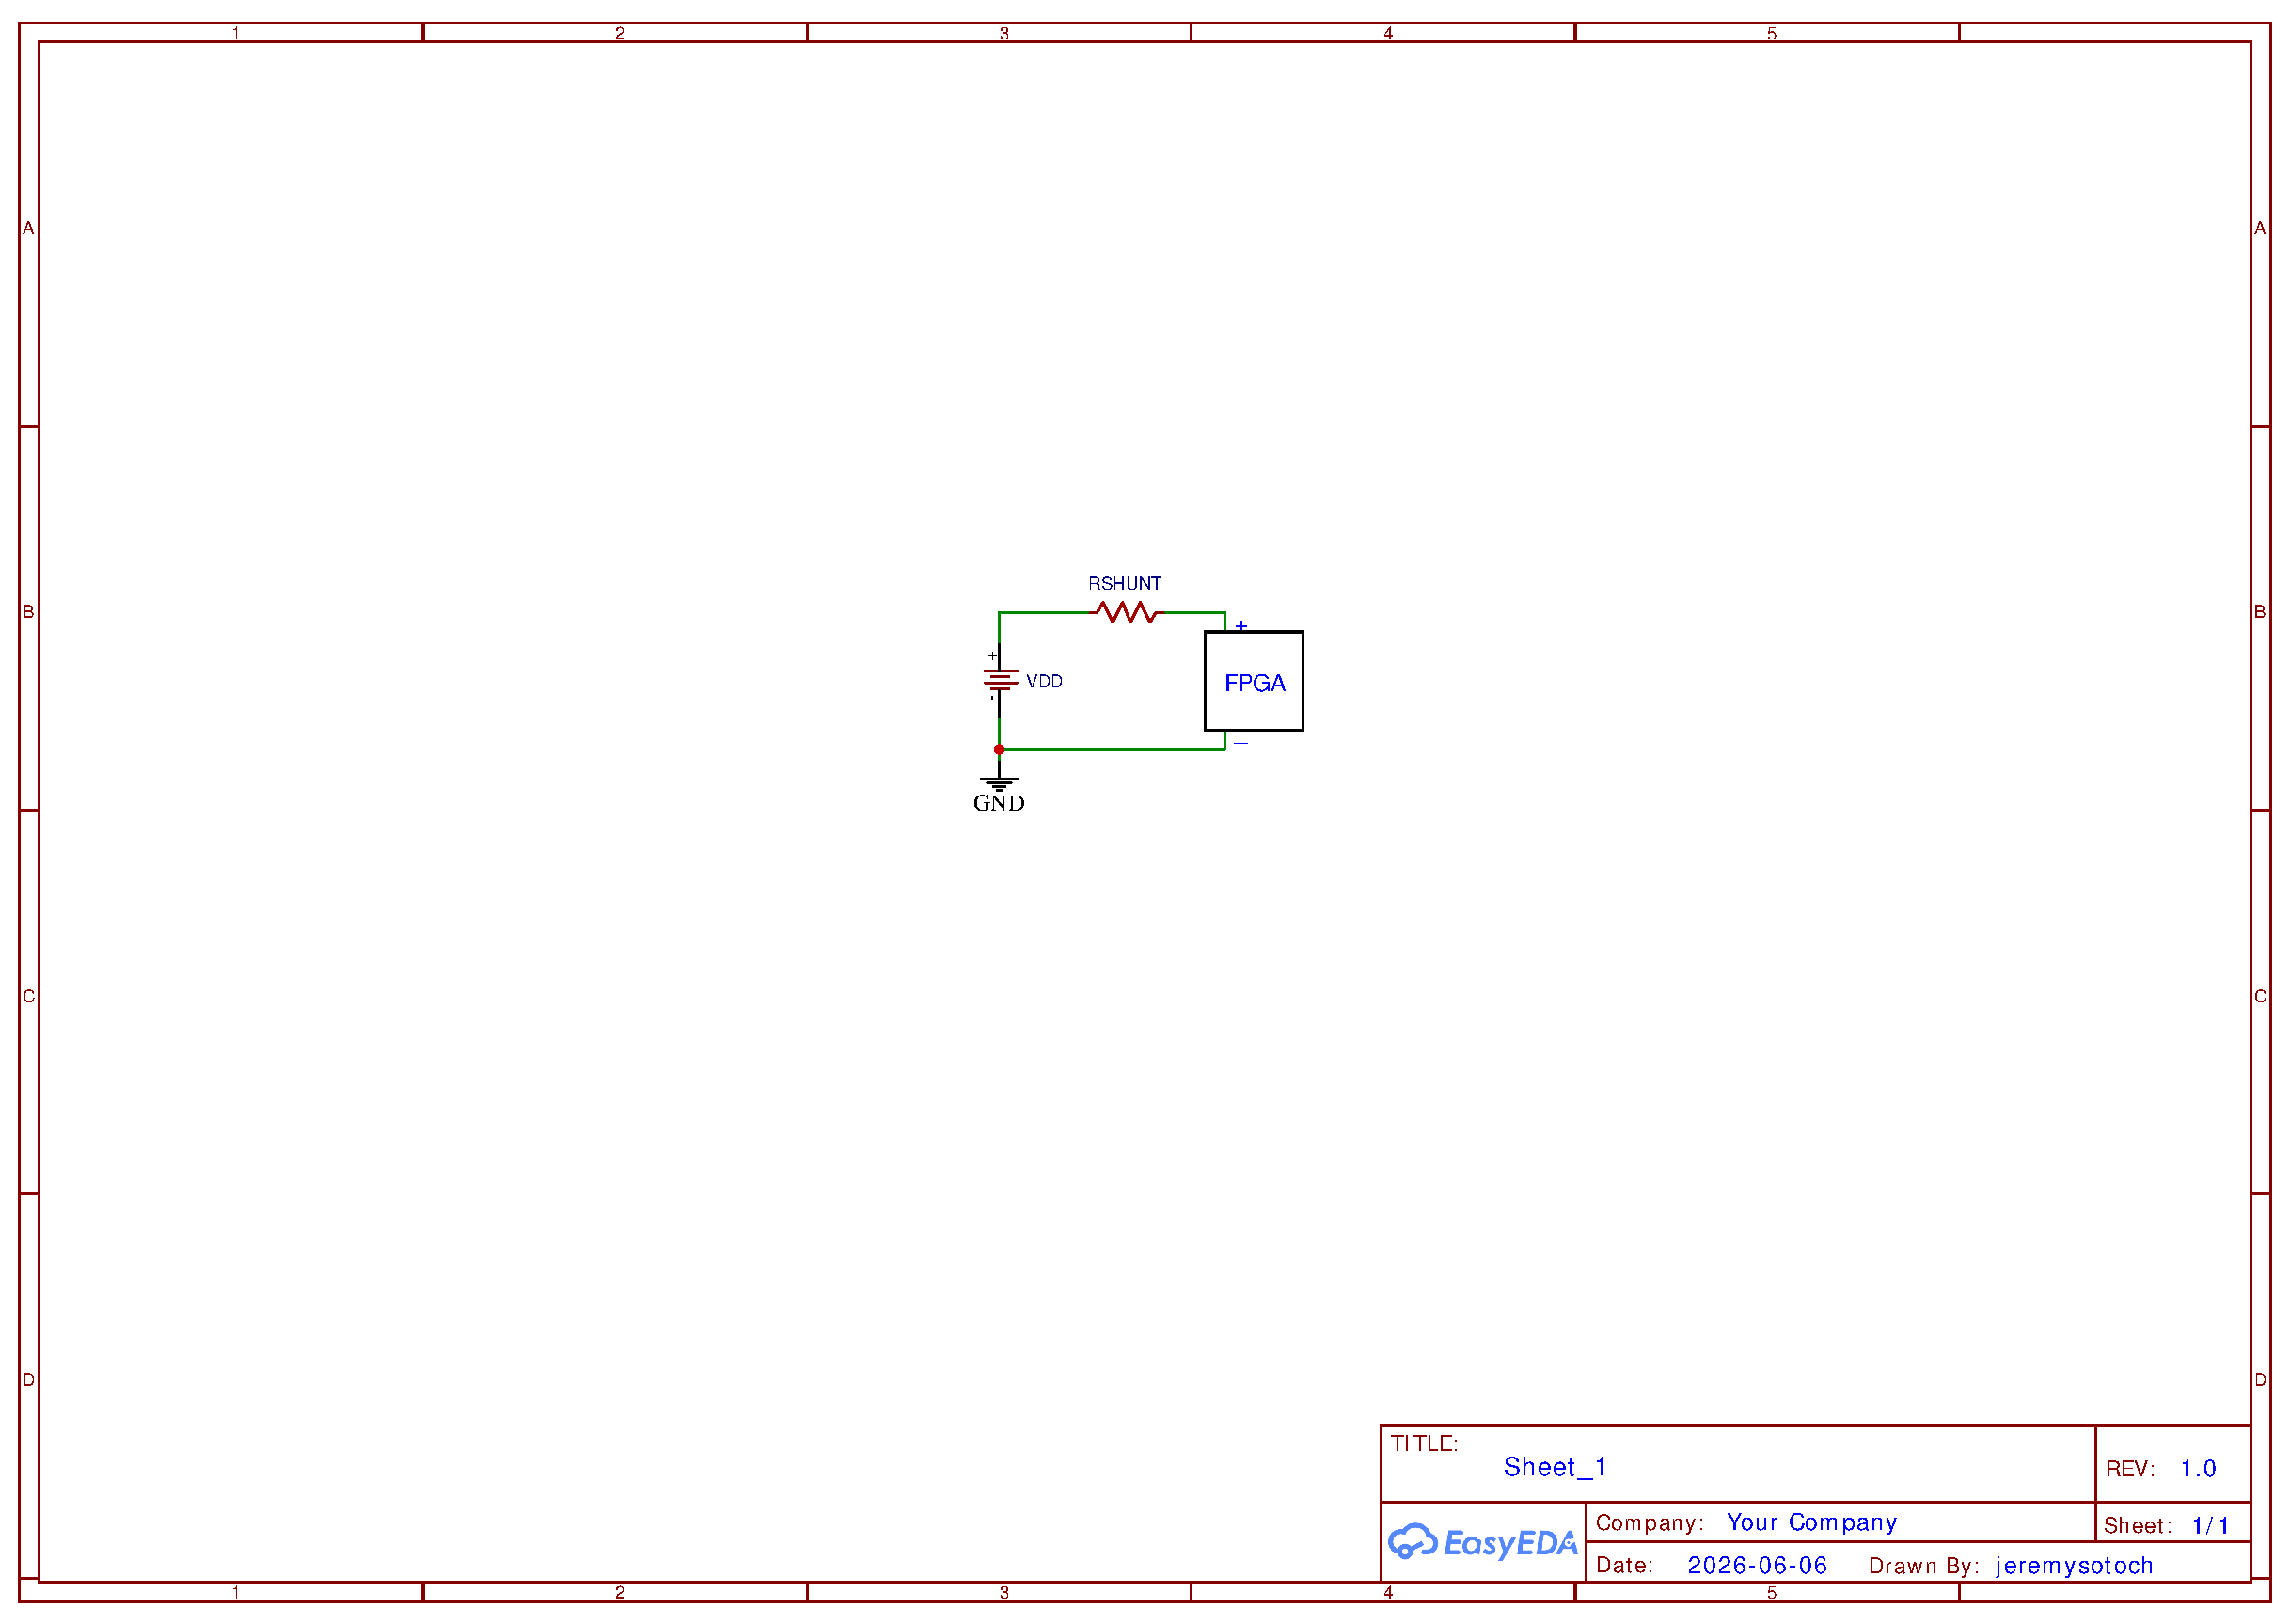
\includegraphics[width=0.78\textwidth, height=0.28\textheight, keepaspectratio,
        trim=440pt 370pt 455pt 255pt, clip]{fig/diagrama_3_3_shunt_alimentacion.pdf}
    \caption{Ubicación del resistor de sensado en la línea de alimentación de la plataforma.}
    \label{fig:lazo_alimentacion_shunt}
\end{figure}

El INA240~\cite{ina240ds} se utiliza porque mide caídas diferenciales pequeñas
sobre resistores de sensado en configuración \emph{high-side}. La variante
INA240A1 aporta una ganancia fija de $G = 20$\,V/V, suficiente para llevar la
caída producida por el shunt a un nivel adecuado para el ADS1115 sin saturar la
entrada en el rango de corriente usado para dimensionar la medición.

La salida del INA240 es una tensión proporcional a la corriente consumida:

\begin{equation}
    V_\text{out} = G \cdot V_{R_\text{shunt}} = G \cdot I \cdot R_\text{shunt}
    \label{eq:vout_ina240}
\end{equation}

Despejando la corriente y sustituyendo en la ecuación~\ref{eq:potencia_medida},
la potencia se obtiene directamente de la lectura del ADC:

\begin{equation}
    P = V_{DD} \cdot \frac{V_\text{out}}{G \cdot R_\text{shunt}}
    \label{eq:potencia_vout}
\end{equation}

Con $R_\text{shunt} = 100\,\text{m}\Omega$ y $G = 20$\,V/V, la tensión de salida
queda dada por:

\begin{equation}
    V_\text{out} = 20 \cdot I \cdot 0.1\,\Omega = 2I 
    \label{eq:vout_valores}
\end{equation}

Como ejemplo, una corriente de 400\,mA produciría $V_\text{out} = 0.8$\,V;
para 1\,A se obtiene $V_\text{out} = 2$\,V. Ambos valores quedan dentro del
rango de entrada seleccionado para el sistema de adquisición.

\subsection{Adquisición y promediado}
\label{sec:adquisicion}

La señal $V_\text{out}$ se adquiere con un sistema autónomo compuesto por el
convertidor analógico-digital ADS1115~\cite{ads1115ds} y la tarjeta de
desarrollo LilyGO TTGO LoRa32~\cite{lilygoloRA32}, basada en el microcontrolador
ESP32. El ADS1115 digitaliza la salida del INA240 y la tarjeta de adquisición
almacena las muestras en una microSD para su procesamiento posterior. La
sincronización con la FPGA se realiza mediante un pulso digital generado por el
firmware.


\begin{figure}[H]
    \centering
    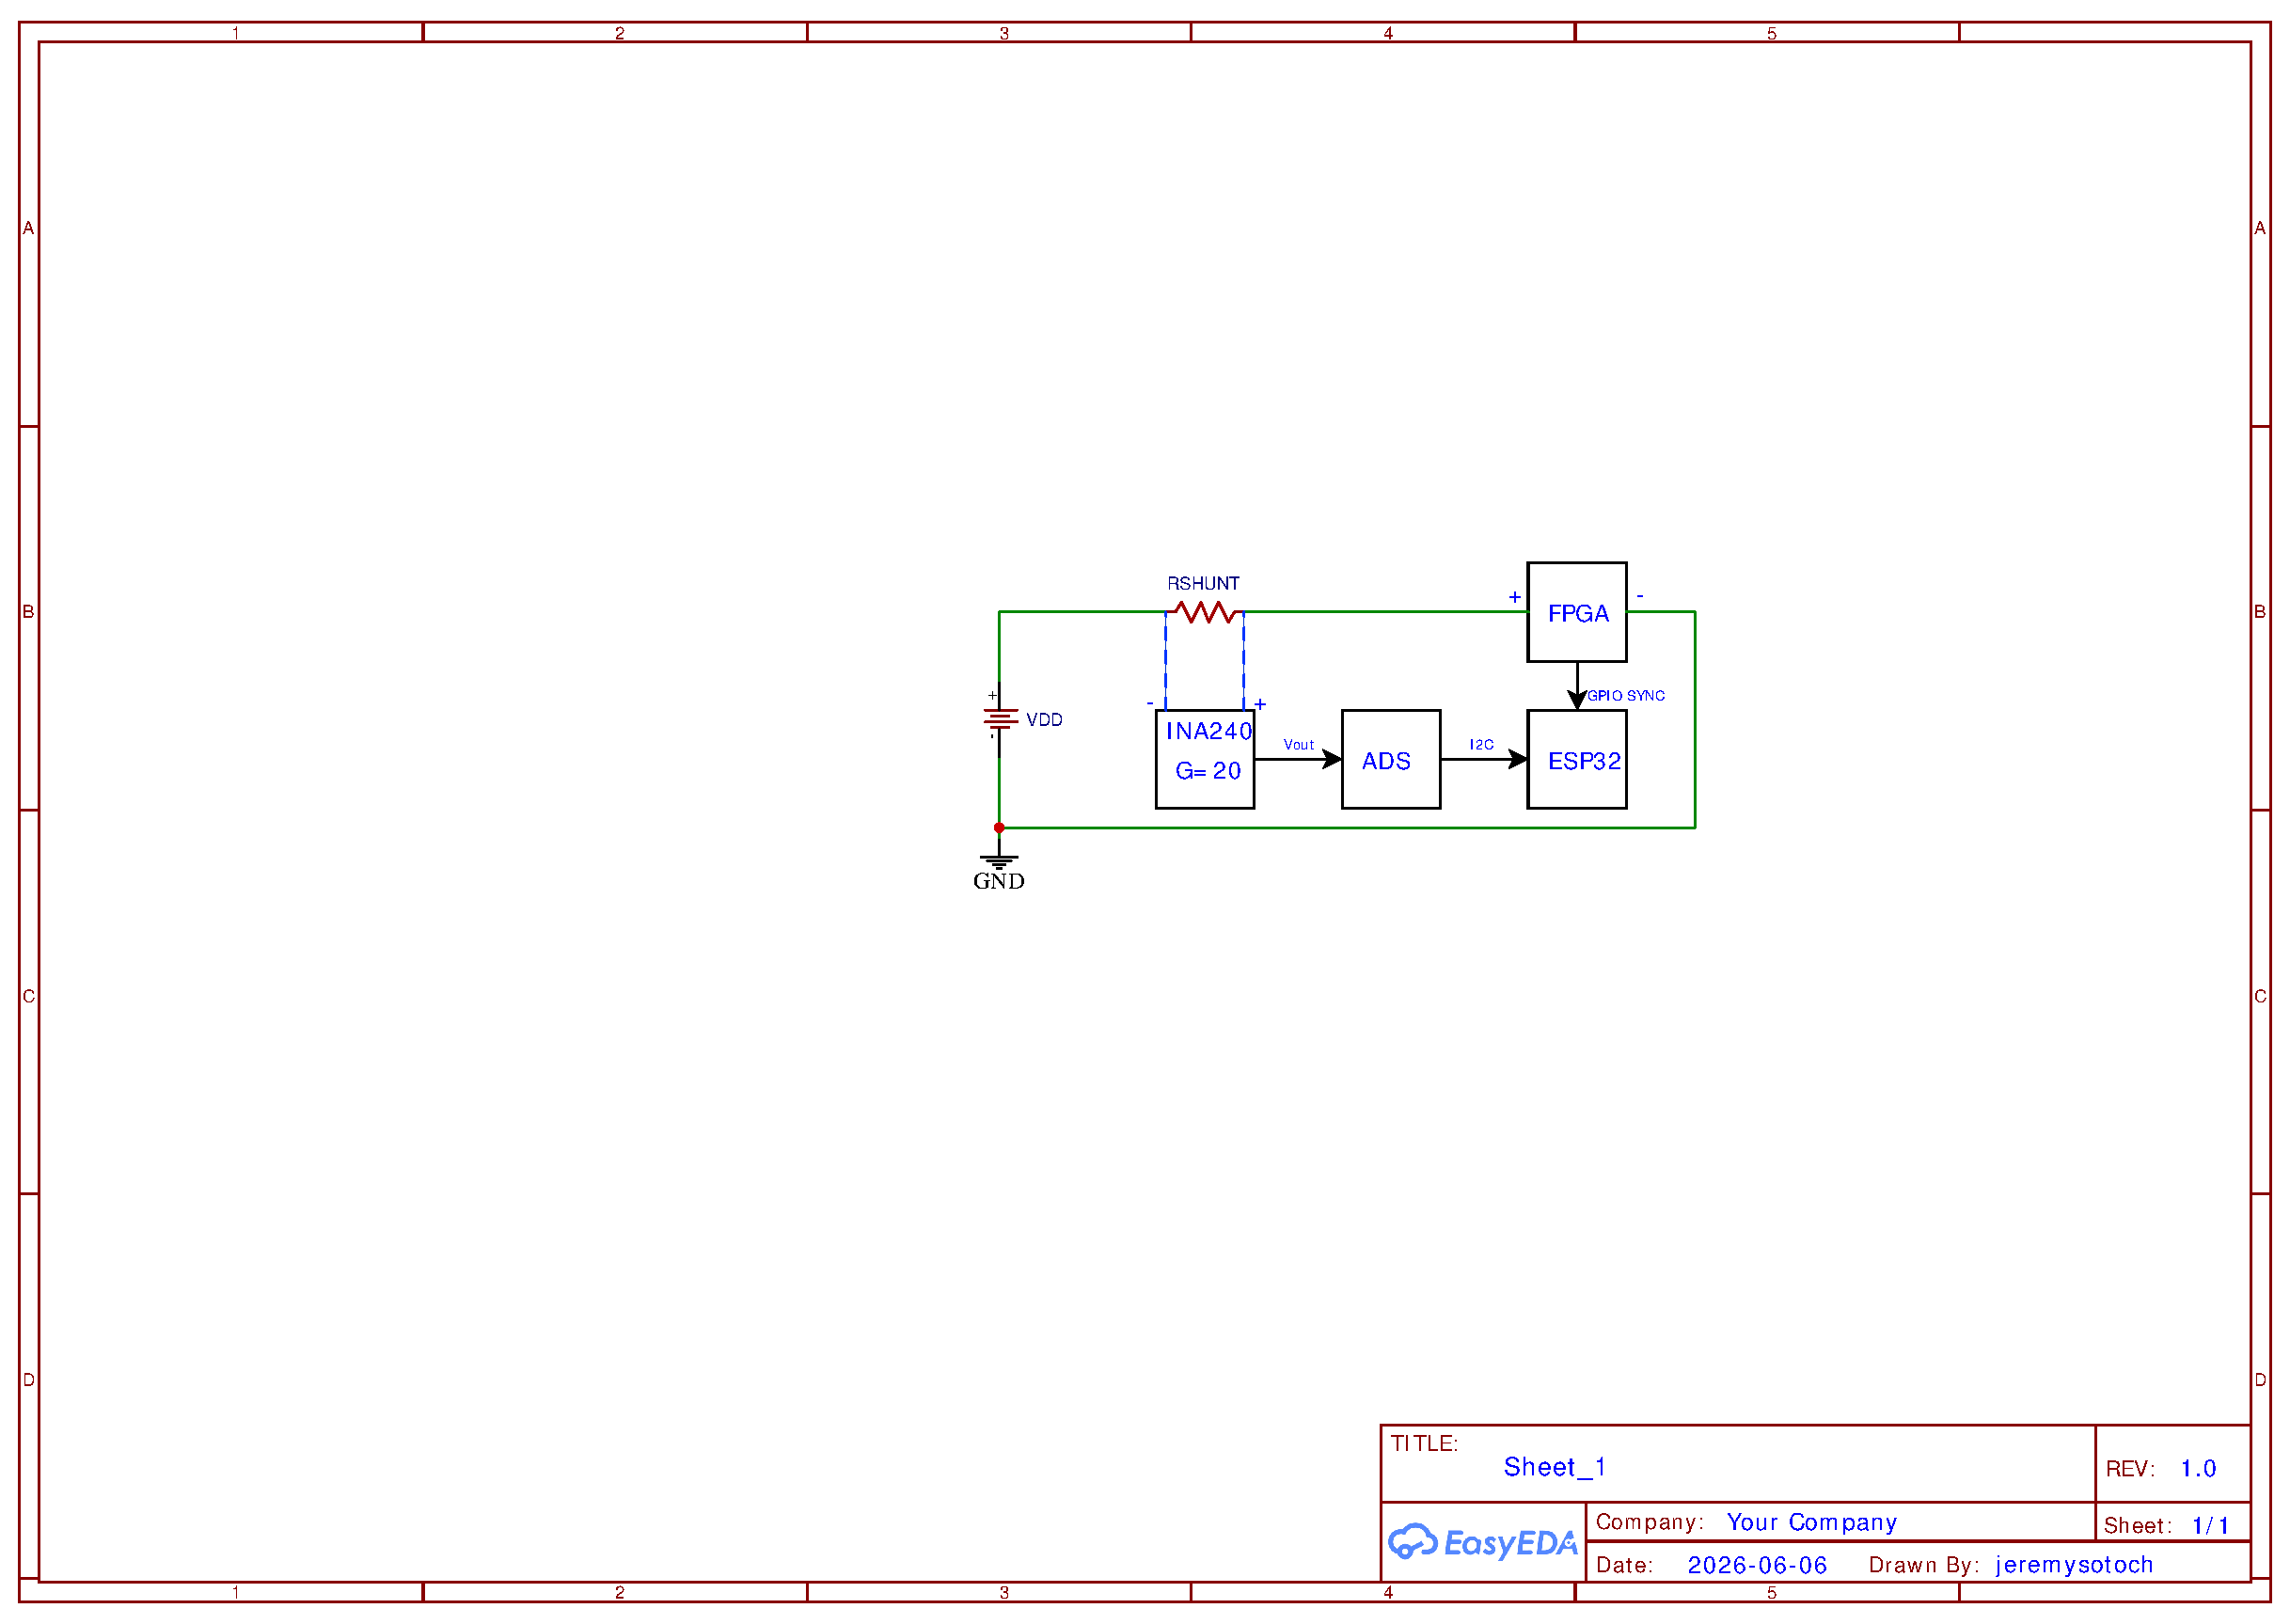
\includegraphics[page=1, width=0.92\textwidth, height=0.30\textheight, keepaspectratio,
        trim=455pt 350pt 285pt 260pt, clip]{fig/diagrama_3_4_cadena_adquisicion.pdf}
    \caption{Cadena de adquisición de potencia desde el resistor de sensado hasta el sistema ESP32.}
    \label{fig:cadena_adquisicion_potencia}
\end{figure}

Se configura inicialmente PGA\,$=\,\pm 4.096$\,V para evitar saturación durante
las pruebas de corriente máxima. Para la caracterización fina se emplea
PGA\,$=\,\pm 2.048$\,V, lo que proporciona una resolución de:

\begin{equation}
    \Delta V = \frac{2 \times 2.048\,\text{V}}{2^{16}} \approx 62.5\,\mu\text{V}
    \label{eq:resolucion_adc}
\end{equation}

equivalente a $31.25\,\mu\text{A}$ de resolución en corriente y $156\,\mu\text{W}$
en potencia a través de la cadena de medición
($R_\text{shunt} = 100\,\text{m}\Omega$, $G = 20$). Esta configuración cubre corrientes de hasta 1\,A ($V_\text{out} = 2$\,V),
valor asociado al consumo máximo de placa reportado para una alimentación de
5\,V~\cite{nexysA7rm}.

La delimitación de la ventana de medición se realizará mediante una señal GPIO
generada por el firmware. Al inicio de la región bajo análisis, el firmware
activará la señal de sincronización; al final de la región la desactivará. La
LilyGO ESP32 detectará ambos flancos para marcar el inicio y el final de las muestras,
de modo que cada ejecución produzca un registro autocontenido asociado a la
región de interés.

El promediado sobre $N$ muestras reduce el ruido aleatorio en un factor
$1/\sqrt{N}$~\cite{ti_current_sensing,fang2021instruction}. Con una tasa de
$860\,\text{SPS}$, las ventanas delimitadas por el pulso de sincronización
proporcionan un número de muestras proporcional a la duración del segmento
medido; para ventanas de 10 a 60 segundos se obtienen entre
$8{,}6\!\times\!10^3$ y $5{,}2\!\times\!10^4$ muestras por ejecución,
suficiente para estimar la potencia promedio de estado estacionario con baja
dispersión. La potencia promedio se calcula a partir del promedio de las
muestras del archivo correspondiente:

\begin{equation}
    \bar{P} = V_{DD} \cdot \frac{\bar{V}_\text{out}}{G \cdot R_\text{shunt}}
            = 5 \cdot \frac{\bar{V}_\text{out}}{20 \cdot 0.1}
            = 2.5\,\bar{V}_\text{out} \quad [\text{W}]
    \label{eq:potencia_promedio}
\end{equation}

donde $\bar{V}_\text{out}$ es el promedio de las muestras consideradas en el
intervalo de medición. La ecuación~\ref{eq:potencia_promedio} asume
$V_{DD}=5\,\text{V}$ constante, despreciando la caída sobre el resistor de
sensado. Para una corriente de 1\,A esta caída es de 100\,mV,
equivalente a una sobrestimación del 2\,\% en la potencia calculada. Como
ejemplo, para 400\,mA la sobrestimación se reduce al
0{,}8\,\%. Cuando el análisis requiere energía total, esta se obtiene
multiplicando la potencia promedio por la duración del intervalo:

\begin{equation}
    E = \bar{P}\,\Delta t
    \label{eq:energia_ventana}
\end{equation}

El intervalo $\Delta t$ podrá obtenerse del reloj interno de la ESP32, usando
los flancos del GPIO como marcas de inicio y fin, o de la diferencia del CSR
estándar \texttt{mcycle} del CV32E40P entre el inicio y el final de la región
medida. La segunda opción ofrece mayor precisión al estar referida al mismo
reloj que ejecuta las instrucciones, por lo que se usará como referencia
temporal en los análisis posteriores.

Esta medición externa se utilizará como referencia para caracterizar y validar el
modelo sobre la plataforma FPGA. Una vez obtenidos los coeficientes, el flujo de
análisis podrá estimar el consumo asociado a una ejecución a partir de los registros CSR, sin repetir la
medición eléctrica para cada región de código analizada.

% -----------------------------------------------------------------------
\section{Módulo clasificador de instrucciones}
\label{sec:modulo_clasificador}

El segundo componente de la solución será un módulo hardware nuevo integrado
directamente en el procesador CV32E40P. Su función será observar las
instrucciones que completen su ejecución en el pipeline, clasificarlas según su
tipo y acumular el conteo en registros accesibles mediante CSR. La estimación no
se calculará dentro del firmware; los conteos se leerán desde el flujo de prueba
y análisis para combinarlos con los coeficientes energéticos caracterizados.

\subsection{Concepto de clasificación}
\label{sec:concepto_clasificacion}

El pipeline del CV32E40P decodifica cada instrucción en la etapa ID antes de
ejecutarla, determinando qué unidades funcionales activará. Esta información
es suficiente para clasificar la instrucción en una de las seis categorías
adoptadas en este trabajo: \emph{Arithmetic}, \emph{Logic}, \emph{Memory},
\emph{Branch}, \emph{Jump} y \emph{Floating point}. Las instrucciones de
carga y almacenamiento se agrupan en \emph{Memory} porque ambas activan la
unidad de carga/almacenamiento, la ALU para el cálculo de dirección, el bus
TCDM y el banco de registros.

El módulo observará las señales que el pipeline genera para una instrucción
válidamente contabilizable, de forma que no se incluyan instrucciones anuladas
por stalls, saltos o vaciados del pipeline. La Tabla~\ref{tab:senales_clas} resume,
para cada categoría, el origen de la señal de clasificación. Las categorías
\emph{Memory}, \emph{Branch} y \emph{Jump} se identifican a partir de las
señales de evento ya generadas por el procesador para los contadores de
rendimiento hardware: \texttt{mhpmevent\_load}, \texttt{mhpmevent\_store},
\texttt{mhpmevent\_branch} y \texttt{mhpmevent\_jump}. La categoría
\emph{Floating point} se identifica con la habilitación \texttt{apu\_en},
asociada a la ruta APU/FPU del núcleo. Las categorías \emph{Arithmetic} y
\emph{Logic} comparten la habilitación \texttt{alu\_en}, por lo que el módulo
las discrimina combinando \texttt{alu\_en} con el código \texttt{alu\_operator}
generado por el decodificador: cuando la operación corresponde al subconjunto
aritmético (sumas, restas, comparaciones, división y resto) se contabiliza
como \emph{Arithmetic}, y cuando corresponde al subconjunto lógico
(\texttt{and}, \texttt{or}, \texttt{xor}, desplazamientos y operaciones de
manipulación de bits) se contabiliza como \emph{Logic}. Las instrucciones de
multiplicación, detectadas mediante \texttt{mult\_en}, también se asignan a
\emph{Arithmetic}. En todos los casos la clasificación se habilita únicamente
cuando la instrucción ha sido retirada, usando la señal
\texttt{mhpmevent\_minstret}. De este modo no se contabilizarán instrucciones
anuladas ni intentos de ejecución que no llegan a completarse. Adicionalmente,
el conteo se inhibirá cuando la instrucción retirada corresponda a un acceso
CSR, identificado mediante la señal \texttt{csr\_access\_ex}: el decodificador
del CV32E40P deja activa la ALU para \texttt{csrr}, \texttt{csrw}, \texttt{csrs}
y \texttt{csrc}, lo que llevaría a contabilizar estas instrucciones como
\emph{Arithmetic}. Filtrarlas evitará que las propias lecturas y escrituras de
los contadores contaminen la categoría aritmética durante la medición.

\begin{table}[H]
\caption{Categoría de instrucción y origen de la señal usada para
clasificarla en el pipeline del CV32E40P.}
\label{tab:senales_clas}
\centering
\begin{tabularx}{\textwidth}{p{2.7cm}p{4.3cm}X}
\toprule
\textbf{Categoría} & \textbf{Condición de detección} & \textbf{Detalle} \\
\midrule
Arithmetic     & \texttt{mult\_en} o \texttt{alu\_en} con \texttt{alu\_operator} aritmético &
Multiplicaciones del multiplicador entero u operaciones aritméticas de la ALU
(\texttt{add}, \texttt{sub}, \texttt{slt}, \texttt{mul} y \texttt{div}). \\
Logic          & \texttt{alu\_en} con \texttt{alu\_operator} lógico &
Subconjunto lógico del decodificador de la ALU
(\texttt{and}, \texttt{or}, \texttt{xor}, etc). \\
Memory         & \(\texttt{mhpmevent\_load}\) o \texttt{mhpmevent\_store} &
Eventos de carga y almacenamiento ya generados por el core
(\texttt{lw}, \texttt{sw}, etc.). \\
Branch         & \texttt{mhpmevent\_branch} &
Evento de salto condicional retirado, generado por la lógica interna del core (\texttt{beq}, \texttt{bne}, etc). \\
Jump           & \texttt{mhpmevent\_jump} &
Evento de salto incondicional retirado, correspondiente a \texttt{jal/jalr}. \\
Floating point & \texttt{apu\_en} &
Habilitación de la unidad de coprocesador (FPU/Xpulp). \\
\bottomrule
\end{tabularx}
\end{table}

\subsection{Contadores e interfaz CSR}
\label{sec:contadores_csr}

Por cada categoría existirá un contador de 64 bits que almacenará el conteo
acumulado de instrucciones retiradas de ese tipo. A la frecuencia de operación
prevista para el SoC sobre la FPGA, del orden de 10\,MHz, un contador de
32 bits dominado por una sola categoría se saturaría tras aproximadamente
siete minutos de ejecución sostenida, margen insuficiente para acumular el
conteo de varias ejecuciones consecutivas sin reinicio intermedio o para
operar el diseño a frecuencias de síntesis mayores. Cada vez que el pipeline complete una instrucción de una
categoría, la lógica del módulo incrementará el contador correspondiente.

Como el CV32E40P es un procesador de 32 bits, cada contador de 64 bits se
expondrá mediante dos CSR personalizados de 32 bits: una palabra baja y una
palabra alta. Estos CSR se ubicarán en el espacio de direcciones reservado por
la especificación RISC-V para implementaciones de modo máquina~\cite{riscvspec}.
El acceso usará las instrucciones estándar de la ISA, sin requerir sistema
operativo ni llamadas al sistema. Las lecturas \texttt{csrr} permitirán
reconstruir el conteo acumulado de cada categoría desde el flujo de prueba,
mientras que escribir cero en ambos CSR reiniciará el contador correspondiente.
De esta forma, una región específica de código podrá delimitarse sin reiniciar
el procesador completo.

\subsection{Integración en el procesador}
\label{sec:integracion_soc}

El módulo se integrará como un bloque independiente dentro del núcleo
CV32E40P, sin alterar la semántica de ejecución del pipeline. En el árbol RTL
del procesador, el módulo se instanciará en \texttt{cv32e40p\_core.sv} junto al
resto de las unidades funcionales, y recibirá como entradas señales ya
disponibles en
el núcleo: \texttt{mhpmevent\_minstret}, \texttt{mhpmevent\_load},
\texttt{mhpmevent\_store}, \texttt{mhpmevent\_branch},
\texttt{mhpmevent\_jump}, además de \texttt{alu\_en},
\texttt{alu\_operator}, \texttt{mult\_en} y \texttt{apu\_en}. Estas señales
permitirán reutilizar la información interna del procesador sin introducir una
nueva etapa de decodificación.


\begin{figure}[H]
    \centering
    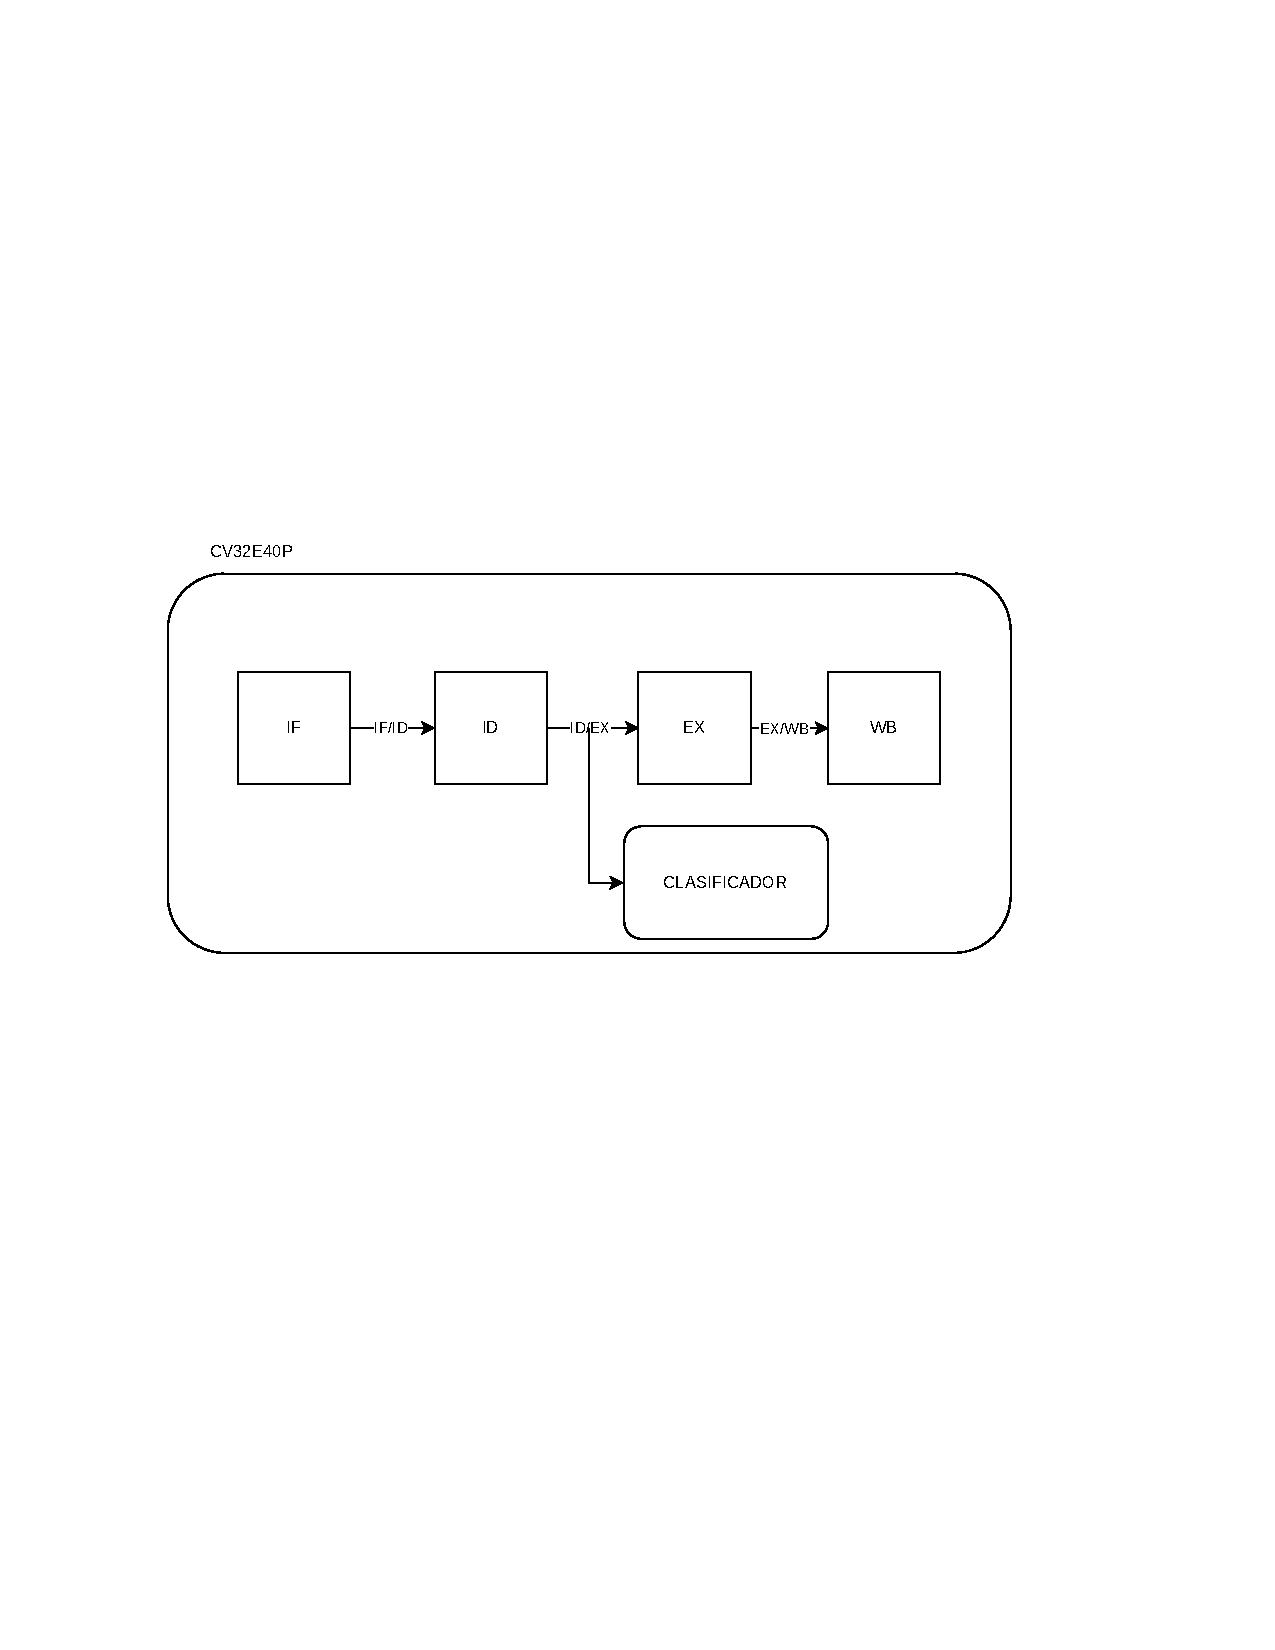
\includegraphics[width=0.95\textwidth, height=0.30\textheight, keepaspectratio,
        trim=80pt 320pt 100pt 245pt, clip]{fig/diagrama_3_5_integracion_clasificador.pdf}
    \caption{Integración conceptual del módulo clasificador como observador del pipeline del CV32E40P.}
    \label{fig:integracion_clasificador_pipeline}
\end{figure}

La integración con los CSR se realizará también en \texttt{cv32e40p\_core.sv}.
En lugar de modificar el bloque \texttt{cv32e40p\_cs\_registers.sv} para que
almacene directamente los contadores del clasificador, se conservará su salida
original en una señal intermedia y se añadirá un multiplexor de lectura. Cuando
la dirección CSR solicitada pertenezca al clasificador, el núcleo devolverá el
dato generado por este bloque; en caso contrario, devolverá el valor original
del banco CSR estándar. Las direcciones usadas para los doce CSR del
clasificador serán \texttt{0xBC0--0xBCB}, dentro del espacio reservado para
implementaciones de modo máquina. Con este esquema, el clasificador se
comportará como una extensión del espacio CSR sin modificar el funcionamiento de
registros existentes como \texttt{mcycle} o \texttt{minstret}.

\subsection{Carga del firmware vía JTAG}
\label{sec:comunicacion_jtag}

La carga del firmware al CV32E40P y la verificación del funcionamiento del
módulo clasificador se realizarán mediante la interfaz de depuración JTAG
integrada en el procesador~\cite{ieee1149_1}. La cadena de comunicación,
ilustrada en la Figura~\ref{fig:jtag_chain}, consta de tres elementos:

\begin{figure}[H]
\centering
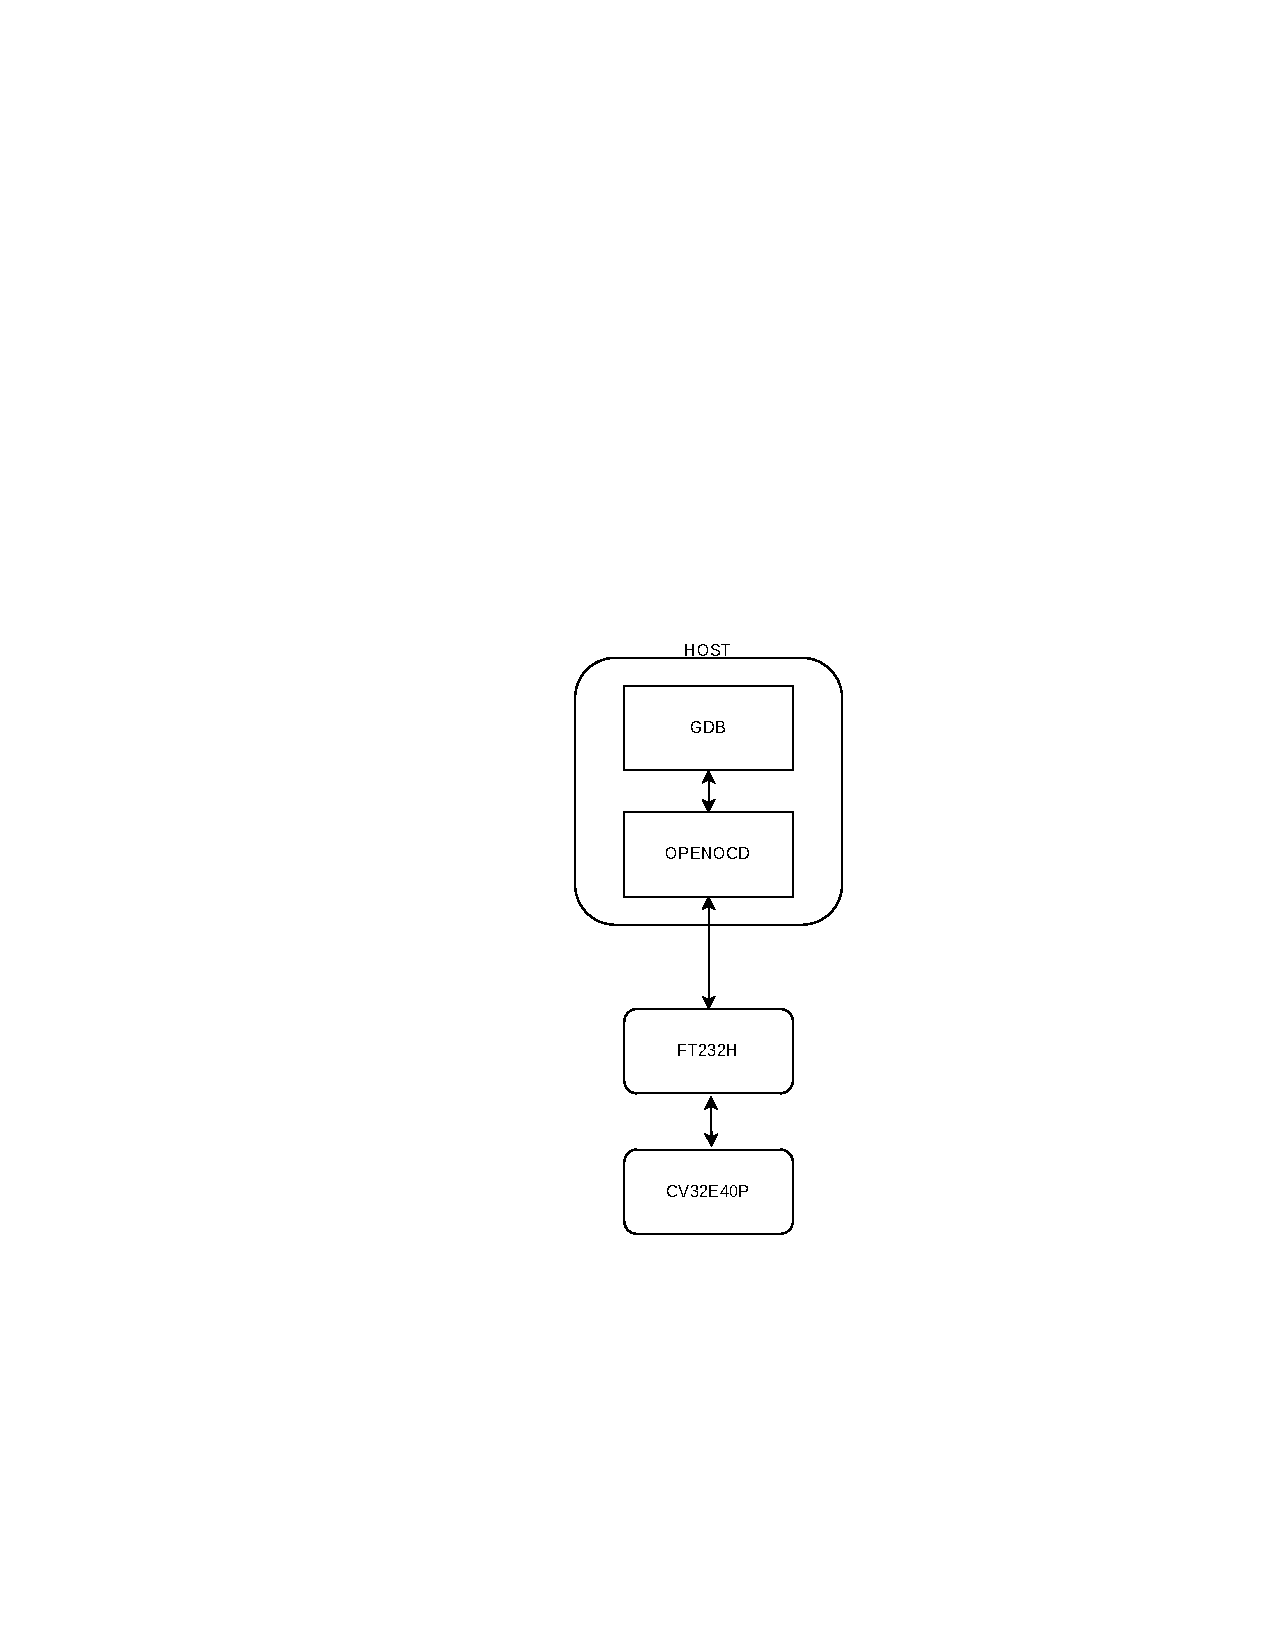
\includegraphics[width=0.32\textwidth, height=0.36\textheight, keepaspectratio,
    trim=270pt 170pt 200pt 280pt, clip]{fig/diagrama_3_6_cadena_jtag.pdf}
\caption{Cadena de comunicación con el CV32E40P.}
\label{fig:jtag_chain}
\end{figure}

El módulo FT232H~\cite{ft232h} actúa como puente entre el puerto USB de la
computadora y las señales JTAG del procesador mediante el motor MPSSE
(\emph{Multi-Protocol Synchronous Serial Engine}). Sobre esta interfaz,
OpenOCD maneja el protocolo JTAG e implementa el acceso definido por la
especificación RISC-V Debug~\cite{openocdmanual,riscvdebugspec}. GDB se conecta
a OpenOCD para cargar el binario en la SRAM del SoC, ejecutar el firmware y
leer los registros CSR del clasificador durante la verificación.

El módulo físico empleado para esta interfaz se muestra en la
Figura~\ref{fig:ft232h_jtag}.


\begin{figure}[H]
    \centering
    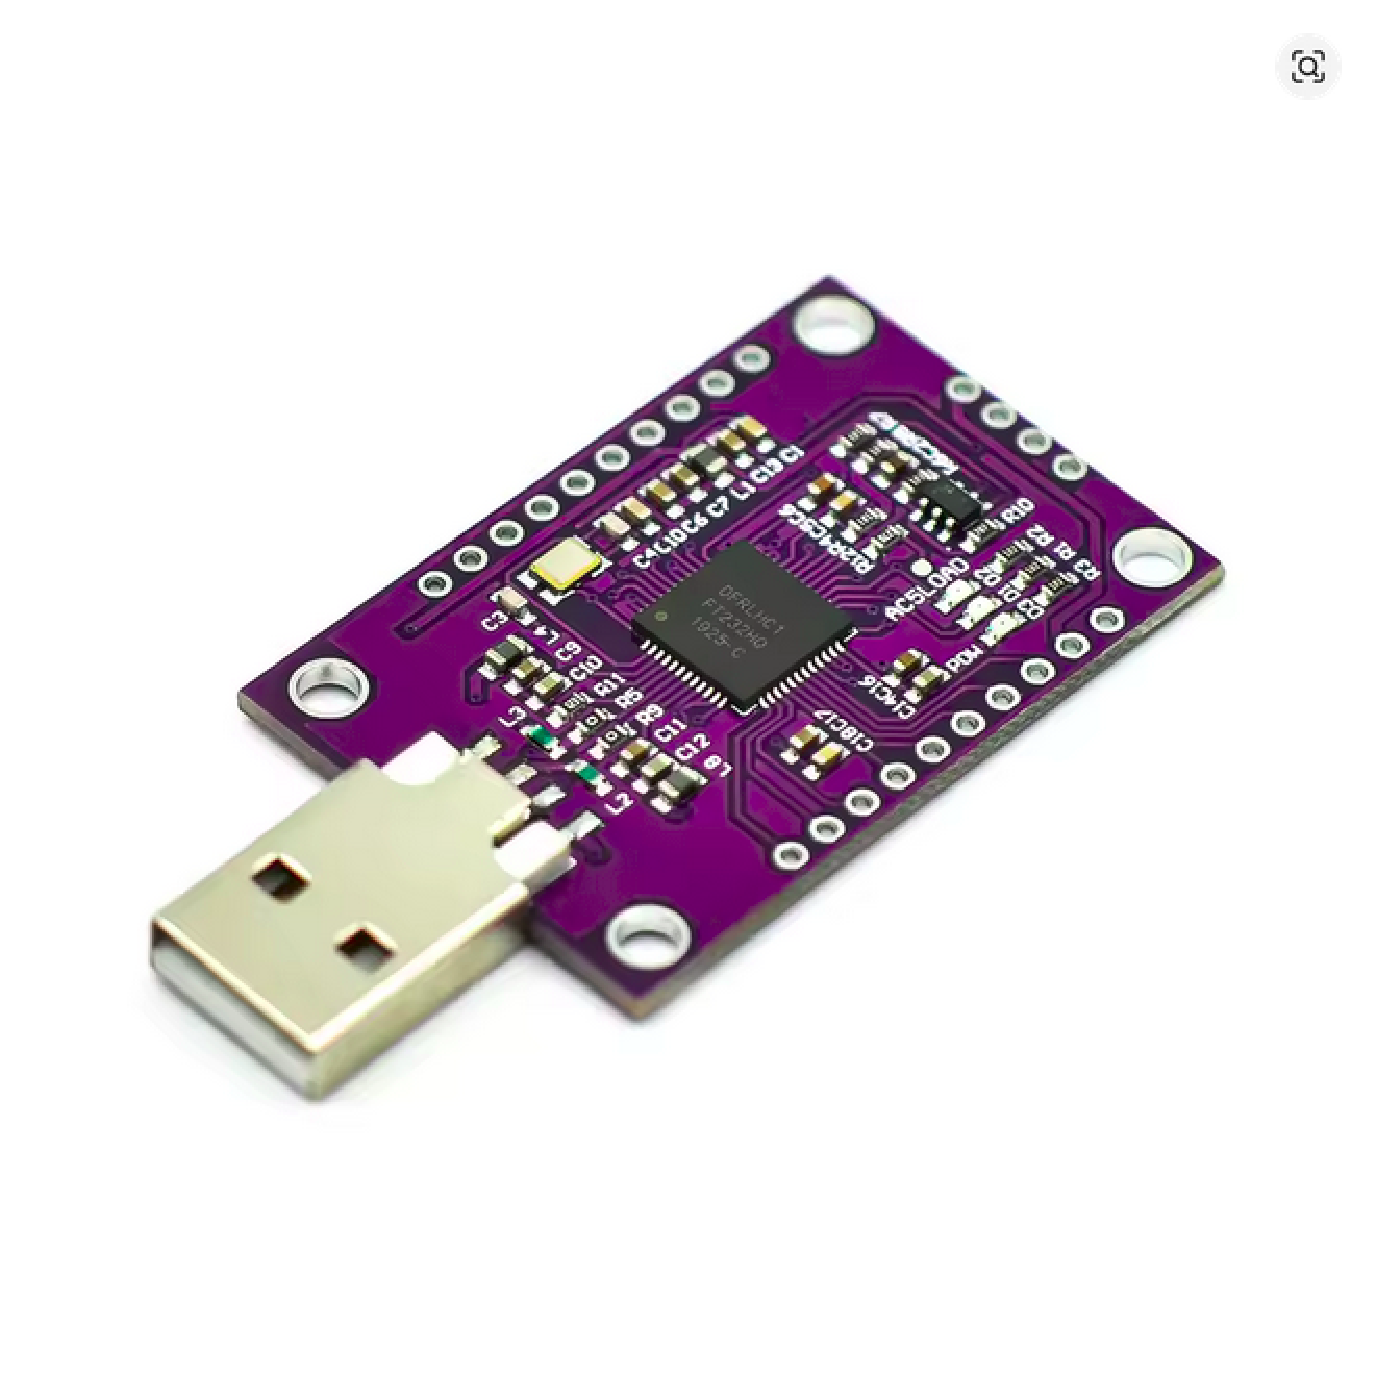
\includegraphics[width=0.40\textwidth]{fig/ft232h_jtag.pdf}
    \caption{Módulo FT232H utilizado como interfaz USB-JTAG.}
    \label{fig:ft232h_jtag}
\end{figure}

% -----------------------------------------------------------------------
\section{Caracterización y estimación}
\label{sec:analisis_datos}

La caracterización de coeficientes energéticos se abordará mediante dos métodos
complementarios. En el método de bucles dominados por categoría, cada programa
de prueba se construirá para que una categoría represente al menos el
95\,\% de las instrucciones ejecutadas. En este caso no será necesario leer los
CSR del clasificador para conocer la categoría dominante, porque el perfil de la
rutina estará definido por construcción. La potencia promedio se obtendrá
mediante una medición en régimen estable durante ventanas de 10 a 60 segundos.

El método de regresión por histograma requerirá que el circuito de medición
(sección~\ref{sec:medicion_potencia}) y el módulo clasificador
(sección~\ref{sec:modulo_clasificador}) operen en conjunto. En ese caso, la
plataforma producirá dos flujos de datos complementarios: las muestras de
potencia registradas por el sistema ADS1115--LilyGO ESP32 en la microSD y los
conteos de instrucciones por categoría leídos de los registros CSR del
procesador. Ambos flujos se combinarán para obtener los coeficientes energéticos
$e_i$ del modelo de estimación, válidos para esta implementación en FPGA.

Ambos métodos producirán un conjunto de coeficientes $e_i$ asociados a cada
categoría de instrucción que posteriormente se compararán según el error de
estimación obtenido frente a las mediciones físicas de referencia, de modo que
la selección final del conjunto de coeficientes dependerá del desempeño
experimental del modelo y no de una preferencia previa por un método
particular.

\subsection{Software de análisis y operación}
\label{sec:scripts_analisis}

El software de apoyo se organizará como un flujo externo de calibración,
validación y operación. Su función será automatizar la ejecución de firmware en
la plataforma, asociar cada ventana de ejecución con las muestras registradas
por el sistema de adquisición y, cuando el clasificador esté integrado, leer los
conteos acumulados en los CSR. A partir de estos datos se calcularán los
coeficientes energéticos del modelo y se generarán los reportes necesarios para
comparar la estimación contra la medición física.

Durante la calibración, el software procesará dos tipos de ejecuciones. En las
rutinas dominadas por categoría, calculará la potencia promedio de cada ventana
y derivará un coeficiente inicial para la categoría correspondiente. En las
cargas mixtas, combinará la energía medida con los histogramas de instrucciones
reportados por el clasificador y resolverá el sistema de regresión descrito en
la sección~\ref{sec:modelo}. La validación posterior usará programas distintos
a los de calibración para comparar la potencia promedio estimada con la potencia promedio medida y
calcular el error relativo del modelo.

Una vez caracterizada la plataforma, el modo de operación final no requerirá la
cadena de medición eléctrica. El usuario ejecutará un firmware sobre el sistema,
el software leerá los conteos por categoría al finalizar la región de interés y
aplicará los coeficientes almacenados para reportar energía, potencia y desglose
por categoría. De esta forma, la instrumentación externa se usará solo durante
la fase de caracterización; la estimación posterior dependerá únicamente del
clasificador integrado y del archivo de coeficientes obtenido experimentalmente.

%%% Local Variables:
%%% mode: latex
%%% TeX-master: "main"
%%% End:
